\documentclass[a4paper,12pt]{article}

\usepackage{graphicx}

\begin{document}

\section{The model}\label{sec-model}
A pandemic is in our case modeled as a dynamic system which likewise
in a very general for is described by:
\begin{equation}
  \frac{d}{dt}X = f(X(t),t,u;\psi), \label{eqn-system}
\end{equation}
where $X(t)$ describes the state of our dynamic system at time
$t$. $u$ in general describes the actuation or control that allows us
to manipulate the syste, and $\psi$ the parameters, that allow one
either to generalize the system, or fit a generalized system to a
specific case. The function $f$ as such describes the complete
dynamics of the system and allows us to understand the evolution of
the system. In our case the vector $X$ is described by compartments of
susceptible, infected but non contaigious, infected and contaigious and
vaccinated population, and the flow between these compartments is
governed by $f$. $u$ in our case are vaccination and non
pharmaceutical interventions that are modelled in our system. $\psi$
in general are the rate constants that link the different compartments
that we either guess, measure or fit. Modelling the system is
challenging as we first of all do not know what $f$ might be in
reality and can only make guesses using classical,
compartment models. Second, the system further is probably chaotic in the sense
that small differences in inital conditions yield huge differences as
the system evolves in time. Further the system contains latent
states, that are hard to be measured i.e. an infected, non contaigous
population that can not be measured by SARS-CoV-2 testing.

The current model implemented is goverend by a system of differential
equations (\ref{eqn-governing-system-start}-\ref{eqn-governing-system-end}).
\begin{eqnarray}
  dS_{ij} &=&
  \left[\zeta_{i}V_{ij}+\eta_{i}R_{ij}-S_{ij}\left(\sum_{k=1}^n
    \sum_{l=1}^m
    \epsilon_{ik}\beta_{jlk}I_{kl}+\frac{v_{ij}(t)S_{ij}p_{ij}}{D_{ij}}S_{ij}\right)
    \right]dt,
  \label{eqn-governing-system-start}
  \\
  dE_{ij} &=& \left(S_{ij} \sum_{l=1}^m\beta_{jli}I_{il}-\delta_i
  E_{ij}\right)dt, \label{eqn-bigE}\\
  dI_{ij} &=& (\delta_i E_{ij} - \gamma_i I_{ij})dt, \label{eqn-bigI} \\
  dV_{ij} &=& (v_{ij}(t)\frac{S^2_{ij}}{D_{ij}}p_{ij})-\zeta_{ij}V_{ij})dt, \\
  R_{ij} &=& \frac{N_j}{N}-S_{ij}-E_{ij}-I_{ij}-V_{ij}, \label{eqn-bigR} \\
  D_{ij} &=& S_{ij} + E_{ij} + a_{ij}I_{ij}+\left(1 -
  r\right)R_{ij}, \label{eqn-bigD} \\
  v_{ij}(t) &=& \frac{d}{dt}\frac{L_{ij}}{1+e^{-k_{ij}+(t-t_{ij}')}},
  \label{eqn-governing-system-end}
\end{eqnarray}
with 
\begin{equation}
  \beta_{jlk} = \hat{R}_k(t)\frac{\gamma_k\sigma_{jk} N C_{jl}}{\rho_k N_l},
  \label{eqn-beta}\\
\end{equation}
where, $\rho_k$ is the largest eigenvalue of the matrix:
\begin{equation}
  M^k_{jl}=f_{j}\sigma_{jk}C_{jl}\frac{N_j}{N_l}, \label{eqn-beta-suppl}
\end{equation}
specific for each variant $k$. 
The system is a multicompartment model, simulating $n$ variants and
$m$ age classes. $S$ is representing a susceptible
population, $E$ an intermediate comporatment that considers a latent
population of infected, that is \emph{non contaigious} so far. $I$ shall
consider the population that is infectious and contaigious. Furhter a
compartment $V$ the currently vaccinated and immune population, that
can source from compartment $S$ at rate $\frac{v(t)S p}{D}$,
considering a population that can be still be immunized by
vaccination. $D$ in this rate can be evaluated on the straightforward using
equation \ref{eqn-bigD}, where $a$ is proportion of asymptomatic
cases, and $r$ the dedection (reporting) rate of infected individuals.
Compartment $R$ considers a
population that is effectivly immunized by the fact that it underwent
infection and has recovered from the desease. $\zeta$ and $\eta$ are
as such the immune waning constants for in the case of $\zeta$ the
immune waning after vaccination and $\eta$ the immune waning after
being immunized by infection. Index $i$ descerns different variants
while index $j$ descerns different age classes.
The system total population is $N$
individuals, devided into $N_j$ age groupes, where $N_j$ holds the
population of age classe $j$. As such all compartments can in the
equations only vary on between 0, no individuals are found in such a
state, to 1, all individuals are found in this state. Maybe
counterintuitive at first glance, summing specific compartment
states over the variant index $i$ may yield a number  $>1$ , which
can be attributed to the fact that a person is indeed, for instance,
susceptible to be infected by different variants. $\beta$ describes
the current infection rate which is modelled in equation
(\ref{eqn-beta}). In this equation (\ref{eqn-beta}) $\hat{R}_k(t)$, represents
the current infection rate at moment time $t$, which can vary due to
non pharmaceutical measures taken by the government, i.e. imposing
social distancing measures or wearing masks. The current model however
considers $\hat{R}_k(t)$, at least over a simulated time
interval, to be constant. $\gamma_i$ found in equations
(\ref{eqn-bigI}) and (\ref{eqn-beta}) represents the conversion rate,
the rate at which individuals in the latent compartment $E$ are
transfered to compartment $I$. Vaccination is currently modelled by a
logistic curve as outlined in equation
(\ref{eqn-governing-system-end}). $L$ in this equation represents the
maximum number of vaccines given, $k$ the steepness of the logistic
curve and hance, how fast the population is vaccinated and $t'$ is the
midpoint of the logistic curve and hence the time given that half of
$L$ vaccines are injected. This curve can either be estimated or
fitted to specific age groups or variants. Equation
(\ref{eqn-governing-system-end}) describes the derivative of the number of
vaccines given at a certain moment $t$. 

The variants interact with each other with a modelled cross immunity
defined by the matrix $\epsilon_{ik}$. The different age groups using
a matrix $C$ that models the probablities that persons from different
age classes might encounter each other. Finally $\sigma_{ji}$, part of
$\beta$ as outlined in equation \ref{eqn-beta} represents the
susceptibility for a specific age group $j$ to a variant $i$.

Vaccination is still of concern in this system and a further
discussion has to be made to clarify if equation (\ref{eqn-bigD}) can
be modelled as such. Further it is unclear if the cross imunity and
$\epsilon$ can be written down as such taking vaccination into
account. Recently introduced immune waning $\zeta$, $\eta$ and as such
the importance given to compartments $V$ and $R$ further reopen the
question if vaccination is modelled correct. Further the very vaguely
formulated proportion of asymtotics $a$ and reporting rate $r$ in
equation (\ref{eqn-bigD}). As such we currently do not recommend to
make use of the vaccination code without further modifications. Vaccination
can simply be disabled by setting $L_{ij}$ in equation
\ref{eqn-governing-system-end} to 0. 

\subsection{Integration}
In our current system we have $n$ variants and $m$ age classes. As
such in the current numerical implementation of our system described
in section \ref{sec-model} 

We have implemented a multiequation Runge-Kutta-Fehlberg solver with adaptive
step size and error control. The method that we have implemented uses
the coefficents introduced by Fehlberg outlined in table
\ref{tab-fehlberg}.
\begin{table}
  \begin{tabular}{c|cccccc}
    k & A(k) & B(k,1) & B(k,2) & B(k,3) & B(k,4) & B(k,5) \\
    \hline
    1 & 0 & & & & & \\
    2 & 1/4 & 1/4 & & & &  \\
    3 & 3/8 & 3/32 & 9/32 & & & \\
    4 & 12/13 & 1932/2197 & -7200/2197 & 7296/2197 & & \\
    5 & 1 & 439/216 & -8 & 3680/513 & -845/4104 &  \\
    6 & 1/2 & -8/27 & 2 & -3544/2565 & 1859/4104 & -11/40 \\
    \hline
    & 1 & 2 & 3 & 4 & 5 & 6 \\
    \hline
    C(k) & 25/216 & 0 & 1408/2565 & 2197/4104 & -1/5 & 2/55 \\
    CH(k) & 16/135 & 0 & 6656/12825 & 28561/56430 & -9/50 & 2/55 
  \end{tabular}
  \caption{Coefficients for the Runge Kutta Fehlberg method with
    adaptive step size.}
  \label{tab-fehlberg}
\end{table}
With these coefficients at hand we integrate a system
described by equation (\ref{eqn-system}) like:
\begin{eqnarray}
  k_{1,i}& = &f(t + A(1)\Delta t,X_i)_i\Delta t, \\
  k_{2,i}& = &f(t + A(2)\Delta t,X_i + B(2,1)k_{1,i})_i\Delta t,  \\
  k_{3,i}& = &f(t + A(3)\Delta t,X_i + B(3,1)k_{1,i} + B(3,2)k_{2,i})_i\Delta t, \\
  \vdots& = &\vdots, \\                   
  k_{6,i}& = &f(t + A(6)\Delta t,X_i + B(6,1)k_{1,i} + B(6,2)k_{2,i} +
  B(6,3)k_{3,i}, \nonumber \\
  &+& B(6,4)k_{4,i}+ B(6,5)k_{5,i})_i \Delta t,
\end{eqnarray}
where $X_i$ describe the states of our system. $f_i$ the state
equations that govern our system. The reader may note that $f$ yields
a $i$ results and hance $i$ coefficents $k_{1,i}$ that all have to be
available in order to evaluate $k_{2,1}$ and so on. We further define:
\begin{equation}
  E_{c,i} = X_i+\sum_{l=1}^6k_{l,i}(\mathrm{CH}(l)), \label{eqn-runge-5}
\end{equation}
and
\begin{equation}
  X(t+\Delta t)_i = \sum_{l=1}^5k_{l,i}(\mathrm{C}(l)), \label{eqn-runge-6}
\end{equation}
where $X(t+\Delta t)_i$ are the new states at $t+\Delta t$ if the largest
of the estimated errors, between a 4th (\ref{eqn-runge-5}) and 5th
(\ref{eqn-runge-6}) order integration:
\begin{equation}
  E_{e,i} = \left|E_{c,i}-X(t+\Delta t)_i\right|,
\end{equation}
is smaller than a defined error $E_d$ and hence,
\begin{equation}
  \max(E_{e,i}) < E_d. \label{eqn-rk-error-ineq}
\end{equation}
If the condition is not met, this step is discarted. Further after
each step a new step size is estimated:
\begin{equation}
  \Delta t_{\mathrm{new}} = \Delta t
  \left[\frac{E_d}{2\max(E_{e,i})}\right]^{1/4}. \label{eqn-rk-delta-update}
\end{equation}
Implementation wise the components of $f_i$ are implemented using
the \emph{state\_eqn} structure as defined in
\emph{runge-kutta-fehlberg.h}. For each state $X_i$ one is therefore
required to define a state equation. The \emph{state\_eqn} structure
takes a function pointer, and a pointer with parameters to that
function. As such an arbitrary array of C functions toghether with
their parameters can constituate the evolution $f$ as in equation
(\ref{eqn-system}).

\subsection{Trajectory}
The resulting trajectory can currently be displayed for all states,
and hence compartments that are solved by the methods outlined above.
As the states are not stored equidistant the value at a certain point
in time $t$ can be obtained by interpolation. In order to obtain a
value at any point $t$ first the interval between two evaluated points
is searched. This is done with an efficent implementation of a
bisection search algorithm. In the next step, four calculated points
are considered. The situation is summerized in figure
\ref{fig-interpol},
where we search for a value at location $t_i$ shown with the red line.
\begin{figure}
  \begin{center}
    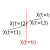
\includegraphics{interpolation.pdf}
  \end{center}
  \caption{Interpolation between 4 points on a trajectory}
  \label{fig-interpol}
\end{figure}

As a quick solution to this problem we have interpolate a polynom of
third order using the four points. Straightforward we solve the system of
equations:
\begin{equation}
  \left[
    \begin{array}{cccc}
      1 & t_1 & t_1^2 & t_1^3 \\
      1 & t_2 & t_2^2 & t_2^3 \\
      1 & t_3 & t_3^2 & t_3^3 \\
      1 & t_4 & t_4^2 & t_4^3 \\
    \end{array}
    \right] \left[ \begin{array}{c}
      c_1 \\
      c_2 \\
      c_3 \\
      c_4 \\
    \end{array}
    \right] = \left[ \begin{array}{c}
      X(t_1) \\
      X(t_2) \\
      X(t_3) \\
      X(t_4) \\
      \end{array}
    \right],
\end{equation}
using the Gauss-Seidel method with the interpolated point being:
\begin{equation}
  X(t_i)=c_1+c_2t_i+c_3t_i^2+c_4t_i^3.
\end{equation}

\section{Input format}

\subsection{Input files}
 
In order to perfom a fit the system needs a \\

\textbf{Model input parameter file:} \\
  A general file that normaly can be passed to the covid model
  solver without a fit. All values in this file serves as inital
  conditions. The file adheres to a keyword - parameters structure
  where a line has to begin with the keyword in question and all
  parameters have to follow space separated on the same line. The
  $n\_variants$ and the $n\_classes$ keywords shall be on top of the
  file as these are needed by the file parsing mechanism in order to
  determine the number of arguments to the following keywords. Table
  \ref{tab-gen-input-parameters} oulines each keyword with the
  parameter format and a description. 

\begin{table}
  \begin{tiny}
  \begin{tabular}{l|l|p{6cm}}
    Keyword & Format & Description  \\
    \hline
    runtime & int & Number of days to simulate \\
    error\_tolerance & float & The error tolerance $E_d$ as in
    equations (\ref{eqn-rk-error-ineq}) and
    (\ref{eqn-rk-delta-update}). \\
    n\_variants & int & The number of variants to consider. \\
    n\_classes & int & The number of age classes to consider. \\
    Rzero & n\_variants*float & The constant $\hat{R}$ value as in
    equation (\ref{eqn-beta}). \\
    variant\_introduction\_date & n\_variants*int & Relative day
    offset of variant introduction. \\
    total\_population & float & The total population to consider \\
    population\_class\_distribution & n\_classes*float & The
    distribution into age classes. \\
    contacts\_between\_classes & n\_classes$^2$*float & The values of
    $C$ as in equations (\ref{eqn-beta}) and (\ref{eqn-beta-suppl}). \\
    reporting\_rate & float & Fraction of cases reported. \\
    asymptomatics\_fraction & n\_classes*n\_variants*float & fraction
    of undetected per age and variant. \\
    initial\_intermediate\_fraction & n\_classes*n\_variants*float &
    Fraction of the total population in $E$. \\
    initial\_infected\_fraction & n\_classes*n\_variants*float &
    Fraction of the total population in $I$. \\
    epsilon & n\_variants$^2$*float & Cross immunity as in equation
    (\ref{eqn-governing-system-start}). \\
    recovery\_rate & n\_variants*float & Recovery rate as of $\gamma$ in
    equation (\ref{eqn-bigI}) \\
    conversion\_rate & n\_variants*float & Conversion rate as of
    $\delta$ in equations (\ref{eqn-bigE}) and (\ref{eqn-bigI}). \\
    pre\_immune\_fraction & n\_classes*float & Proportions of
    primmunized before the start of the simulation. \\
    sigma & n\_classes*n\_variants*float & The susceptibility of a
    certain age group to a certain variant, as of $\sigma$ in
    (\ref{eqn-beta-suppl}).\\
    immune\_drain & n\_variants*float & Rate constant describing the
    loss of immunity from previous infections. As of $\eta$ in equation
    (\ref{eqn-governing-system-start}). \\
    vaccine\_drain & n\_variants*float & Rate constant describing the
    loss of immunity from vaccination. As of $\zeta$ in equation
    (\ref{eqn-governing-system-start}). \\
    vaccine\_logistic\_maximum & n\_variants*n\_classes*float & The
    maximum of the logistic. 
    function describing vaccination. \\
    vaccine\_logistic\_growth & n\_variants*n\_classes*float & The
    speed of vaccination. \\ 
    vaccine\_logistic\_midpoint & n\_variants*n\_classes*float & The
    midpoint of the logistic function describing vaccination \\
    vaccine\_efficiency & n\_variants*n\_classes*float & The
    efficiency of a vaccine towards a variant.
  \end{tabular}
  \end{tiny}
  \caption{The parameters passed to the model found in its input
    file. These are all the parameters needed if a simple model
    simulation is performed, run with \emph{execute\_model}. If a fit
    using \emph{covid\_fit}
    is performed serveral of the parameters are overwritten by either
    the regional data: i.e. total\_population or age distribution, or
    the fit itself: i.e. Rzero.}
  \label{tab-gen-input-parameters}
\end{table}

\end{document}





